\documentclass{beamer}
\usetheme{Madrid}

%Packages BEGIN
\usepackage{amsmath}
\usepackage{physics}
\usepackage{hyperref} 
\usepackage{mathtools} 

%Packages END

% Chinese settings start
\usepackage{xeCJK} % use this package to set Chinese and English font separately
\setCJKmainfont{Noto Serif CJK TC} % Serif font in Ubuntu. Choose the Chinese font available in your device
\setCJKmonofont{Noto Serif CJK TC} % Serif font in Ubuntu. Choose the Chinese font available in your device
\setCJKsansfont{Noto Serif CJK TC} % Serif font in Ubuntu. Choose the Chinese font available in your device
\XeTeXlinebreaklocale "zh" % enabling auto linebreaks
\XeTeXlinebreakskip = 0pt plus 1pt % enabling auto linebreaks 
% Chinese settings end

\usefonttheme[onlymath]{serif} 
\setbeamertemplate{bibliography item}{\insertbiblabel} 

\title[Factorizing 15]{Factorizing 15 Using Shor's Algorithm\\and My Investigation of Error}
\author{Hao-Chien Wang}
\institute[NTUPhys]{Department of Physics, National Taiwan University}

\begin{document}

\begin{frame}
	\titlepage
\end{frame}

\begin{frame}{Outline}
	\tableofcontents
\end{frame}

\section{Review}%
\label{sec:review}

\begin{frame}{Review}
	\begin{figure}[h]
		\centering
		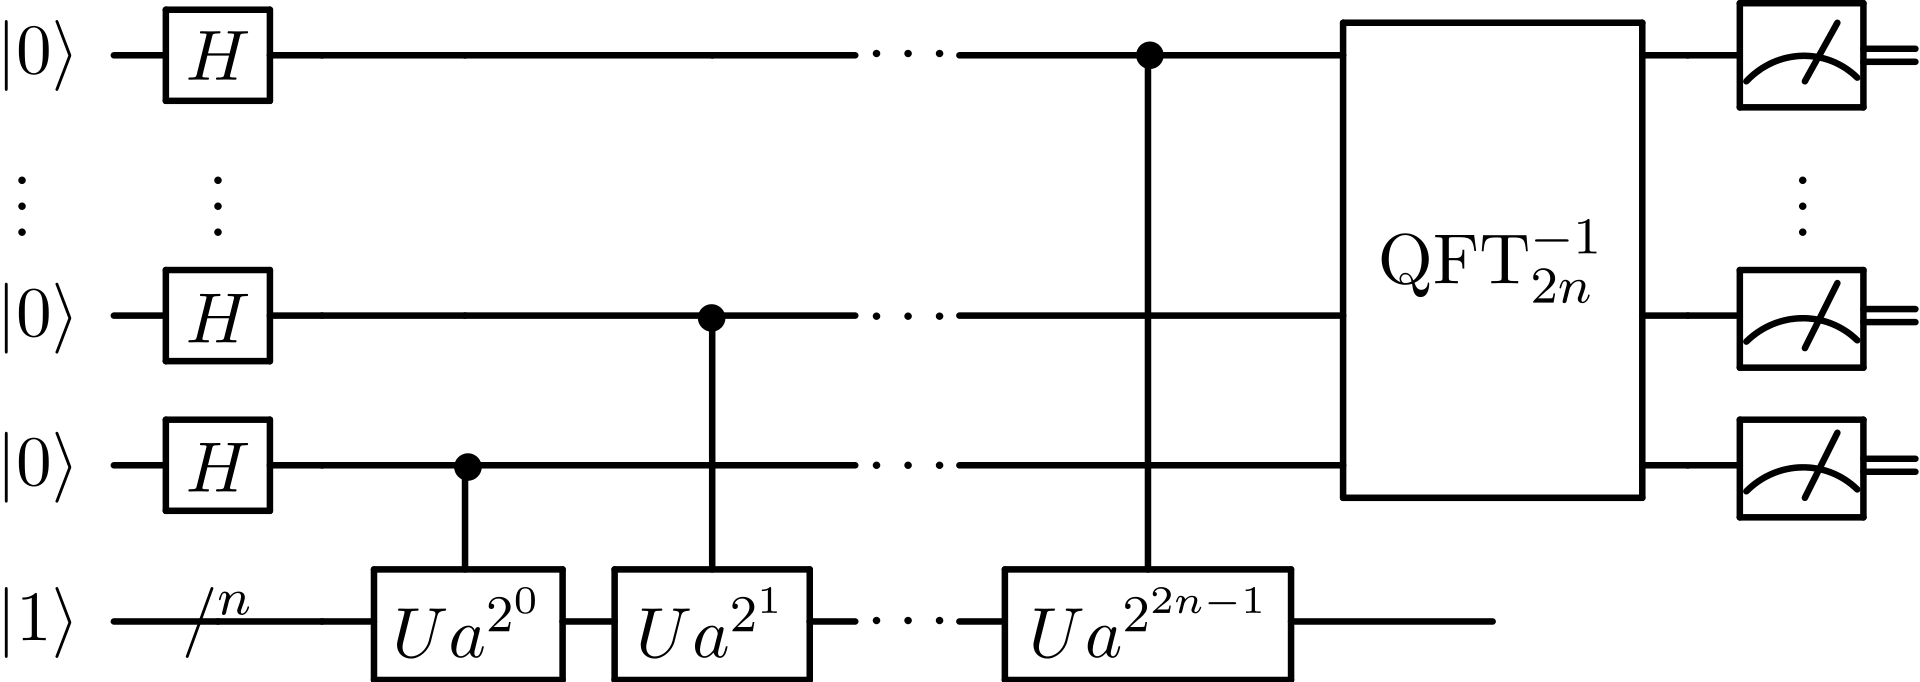
\includegraphics[width=\linewidth]{./figs/simpleshor.png}
		\caption{The circuit of Shor's algorithm.}%
		\label{fig:simpleshor}
	\end{figure}
	
\end{frame}

\section{Method}%
\label{sec:method}

\begin{frame}{Method}
Number of qubits: at least 6.\\
The options of $a$ for $N=15$:
\begin{itemize}
	\item Easy case: 4, 11, 14 ($a^{2^k} \mod N = 1 \: for \: k \geq 1$)
	\item Difficult case: 2, 7, 8, 13 ($a^{2^k} \mod N = 1 \: for \: k \geq 2$)
\end{itemize}
\end{frame}

\subsection{Difficult case}%
\label{sub:difficult_case}

\begin{frame}{Difficult case: Circuit ($a=7$)}

\begin{figure}[h]
	\centering
	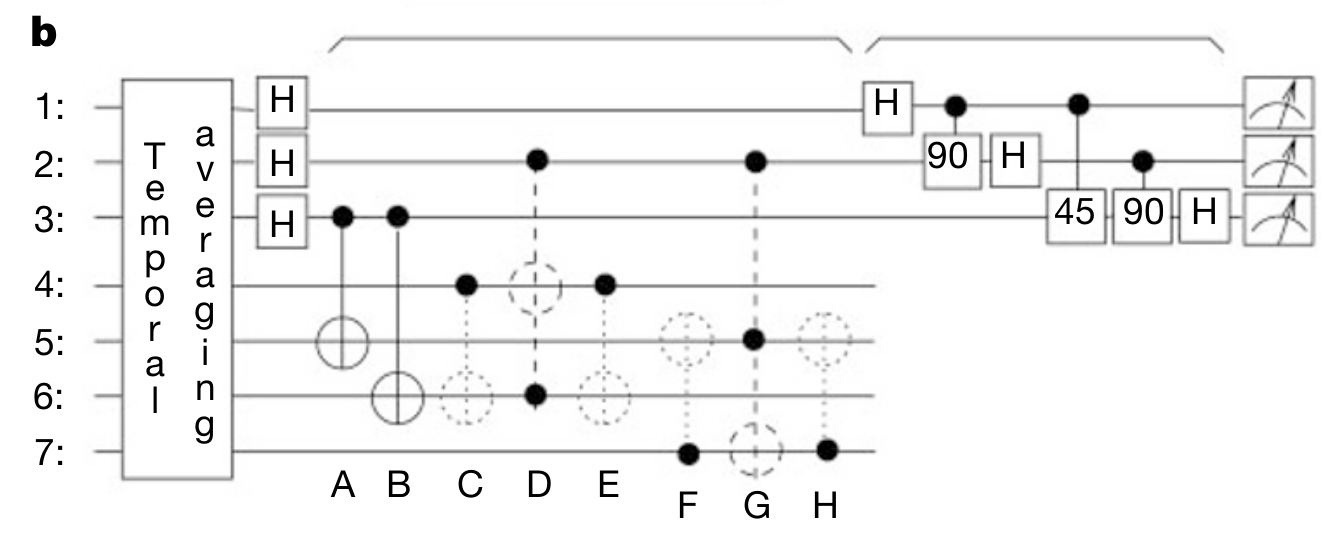
\includegraphics[width=\linewidth]{./figs/7cirucit.png}
\end{figure}
	
\end{frame}

\begin{frame}{The $4n \mod 15$ gate}
	\begin{figure}[h]
		\centering
		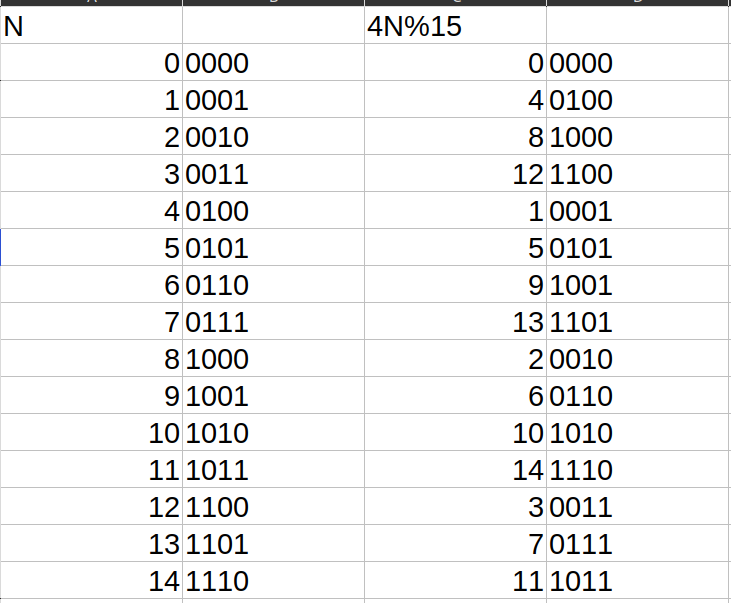
\includegraphics[width=0.6\linewidth]{./figs/times4.png}
	\end{figure}
\end{frame}

\begin{frame}{Gate simplification}
	\begin{equation*}
		\begin{pmatrix}
			1 & 0 & 0 & 0 \\
			0 & 1 & 0 & 0 \\
			0 & 0 & 0 & 1 \\
			0 & 0 & 1 & 0 \\
		\end{pmatrix}
		\begin{pmatrix}
			1 & 0 & 0 & 0 \\
			0 & 0 & 0 & 1 \\
			0 & 0 & 1 & 0 \\
			0 & 1 & 0 & 0 \\
		\end{pmatrix}
		\begin{pmatrix}
			1 & 0 & 0 & 0 \\
			0 & 1 & 0 & 0 \\
			0 & 0 & 0 & 1 \\
			0 & 0 & 1 & 0 \\
		\end{pmatrix}
		=
		\begin{pmatrix}
			1 & 0 & 0 & 0 \\
			0 & 0 & 1 & 0 \\
			0 & 1 & 0 & 0 \\
			0 & 0 & 0 & 1 \\
		\end{pmatrix}
	\end{equation*}
	\begin{figure}[]
		\centering
		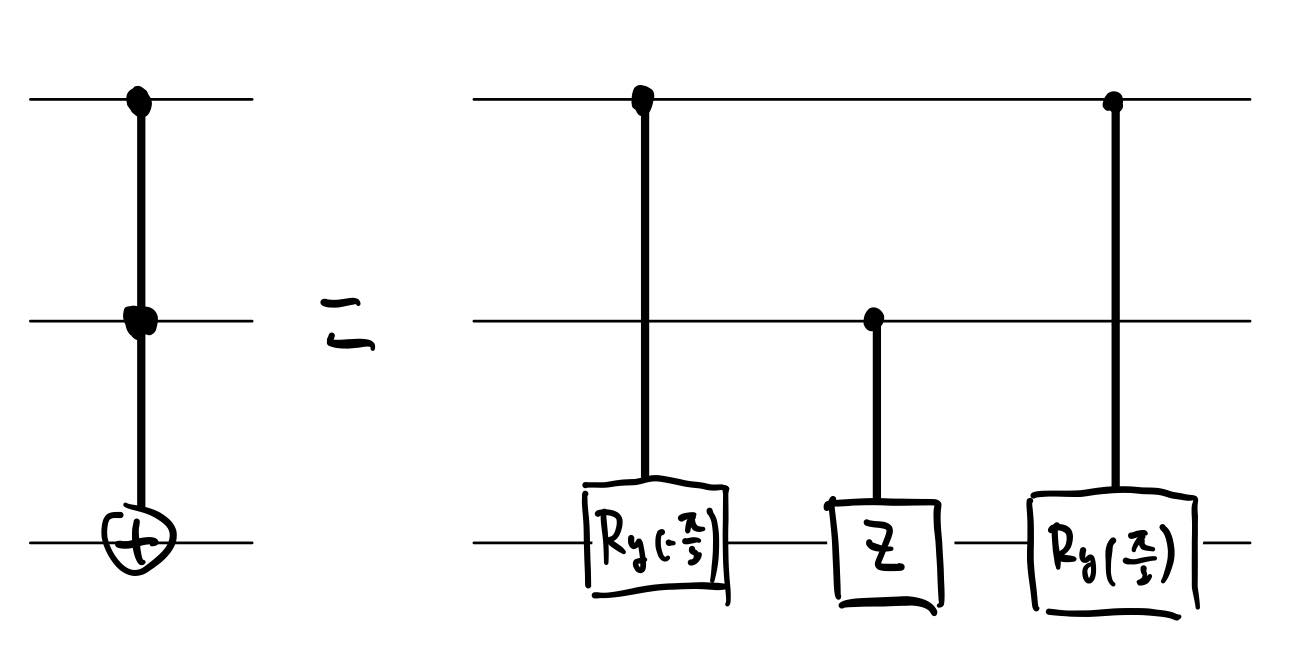
\includegraphics[width=0.5\linewidth]{./figs/toffoli.jpg}
	\end{figure}
	
\end{frame}

\subsection{Easy case}%
\label{sub:easy_case}

\begin{frame}{Easy case: Circuit}
	\begin{figure}[h]
		\centering
		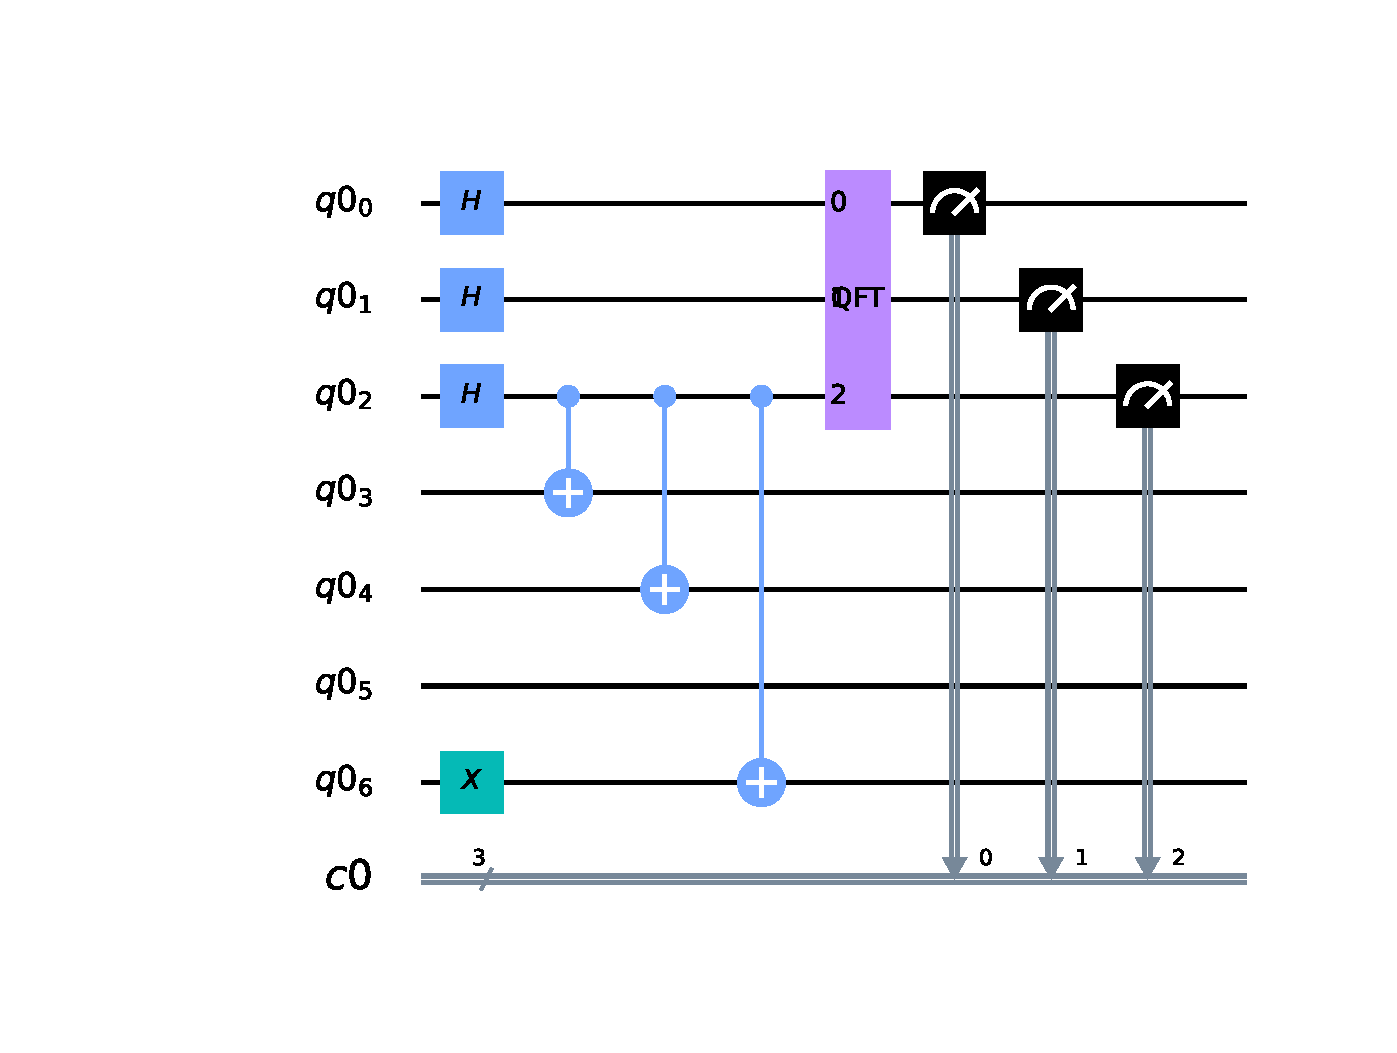
\includegraphics[width=\linewidth]{./figs/11circuit.pdf}
	\end{figure}
\end{frame}


\section{Results}%
\label{sec:results}

\begin{frame}{Result: $a=7$}
	\begin{figure}[h]
		\centering
		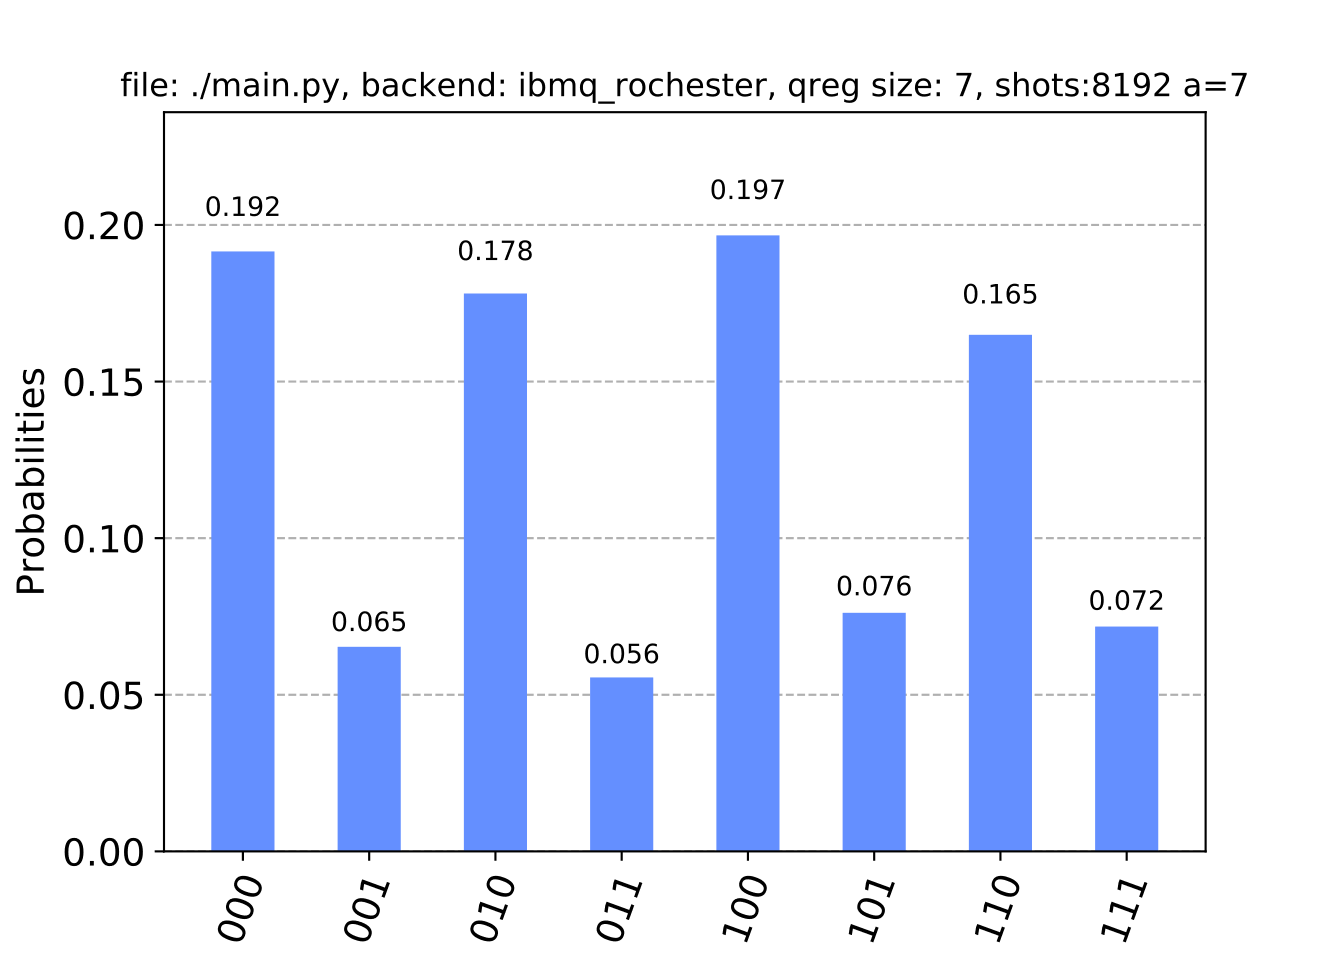
\includegraphics[width=0.8\linewidth]{./figs/15_7.png}
	\end{figure}
\end{frame}

\begin{frame}{Result: $a=11$}
	\begin{figure}[h]
		\centering
		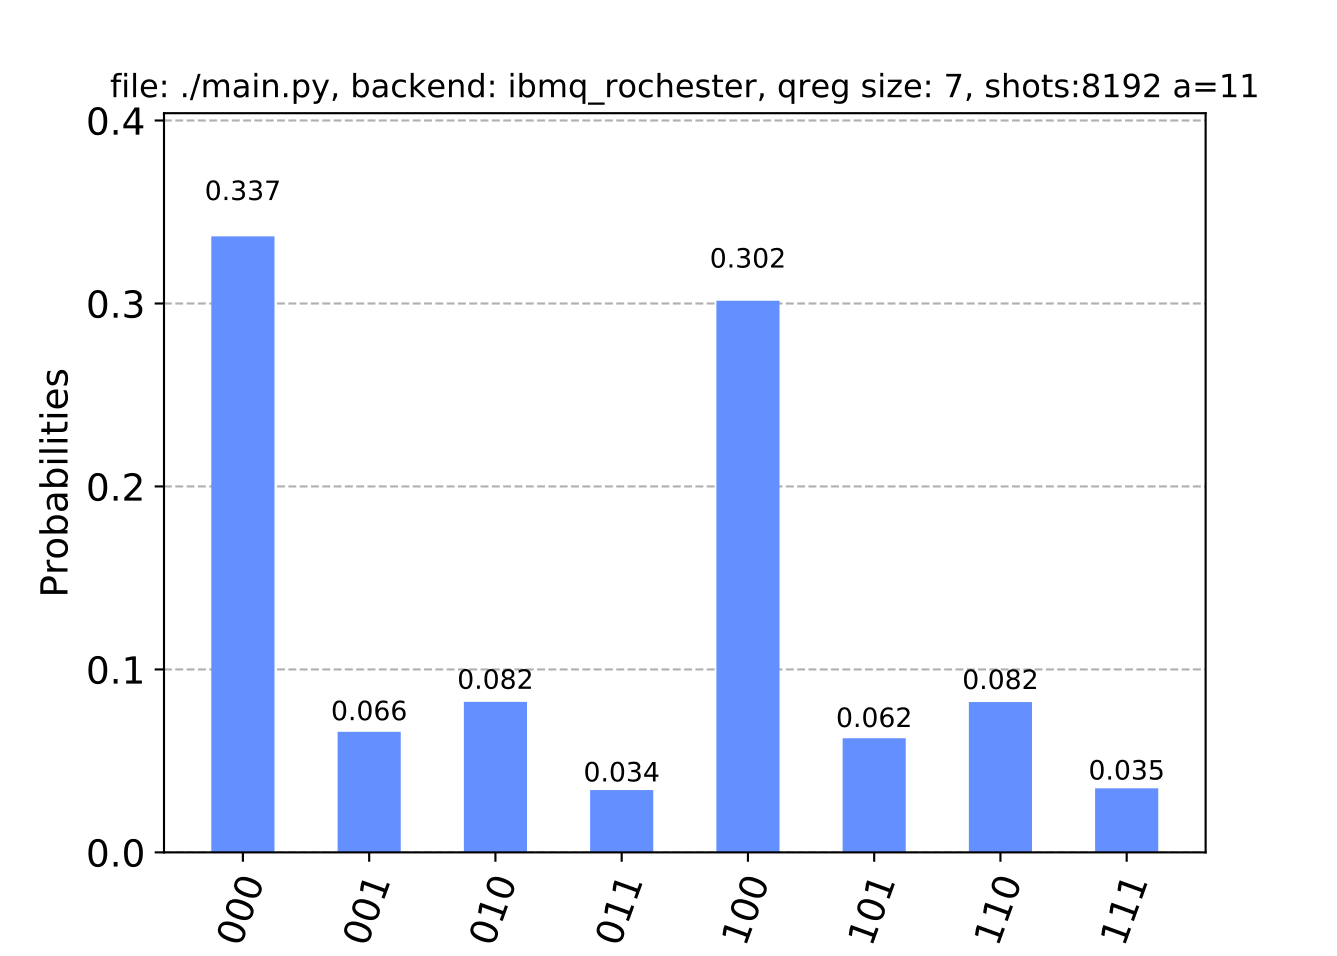
\includegraphics[width=0.8\linewidth]{./figs/15_11.png}
	\end{figure}
\end{frame}
	
\begin{frame}{Result: $a=2$}
	\begin{figure}[h]
		\centering
		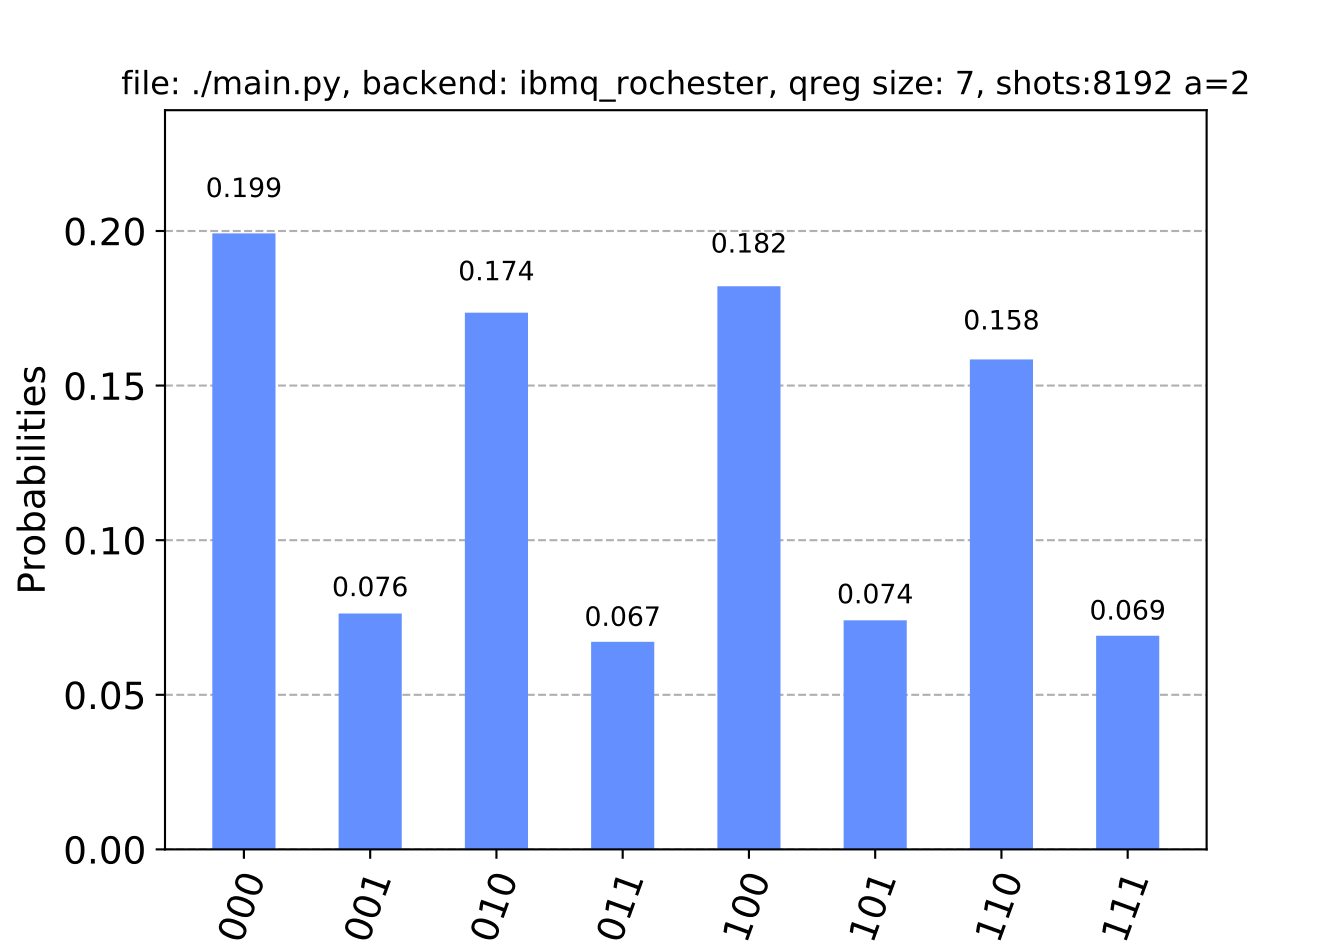
\includegraphics[width=0.8\linewidth]{./figs/15_2.png}
	\end{figure}
\end{frame}

\section{Discussion}%
\label{sec:discussion}

\begin{frame}{Discussion}
	\begin{itemize}
		\item How many qubits do we actually need in the first register?
		\item Do we need to know the answer in advance?
			Yes. While deciding the number of qubits of the first register.
		\item What do we need in order to factorize larger numbers?
			A powerful compiler is required (peephole compiler)
	\end{itemize}
\end{frame}

\begin{frame}{Can we factorize 21?}
	\begin{figure}[h]
		\centering
		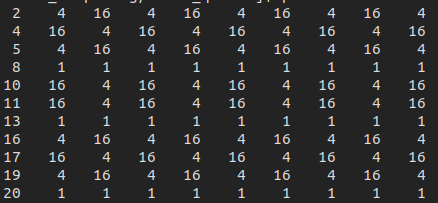
\includegraphics[width=0.8\linewidth]{./figs/21cases.png}
	\end{figure}
	
\end{frame}

\section{Brief discussion on errors}%

\subsection{Measurement error mitigation}%

\begin{frame}{Measurement error mitigation}
		Assuming that there's some probability for each bitstring to flip to 
		another while measured.	
		\begin{equation*}
			C_{noisy} = M C_{ideal}
		\end{equation*}
		$\Rightarrow$Try each bitstring to construct the matrix!
		
\end{frame}

\begin{frame}{Results}
	\begin{figure}[h]
		\centering
		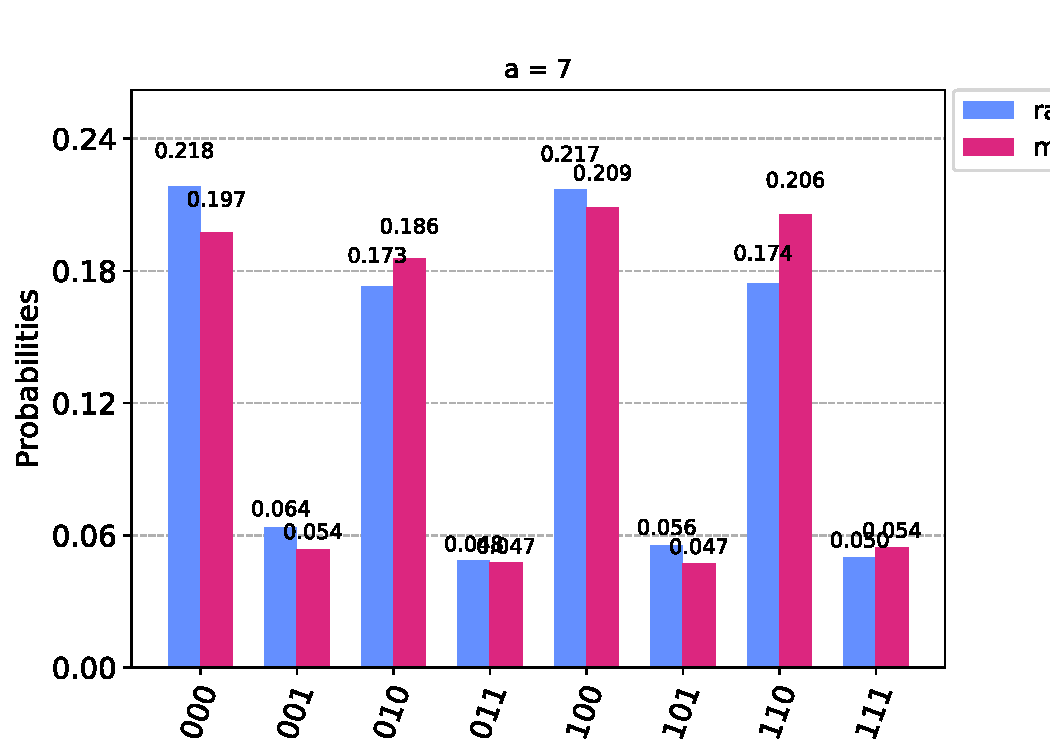
\includegraphics[width=0.8\linewidth]{./figs/error_mitigation_7_cambridge.pdf}
	\end{figure}
\end{frame}

\begin{frame}{Results}
	\begin{figure}[h]
		\centering
		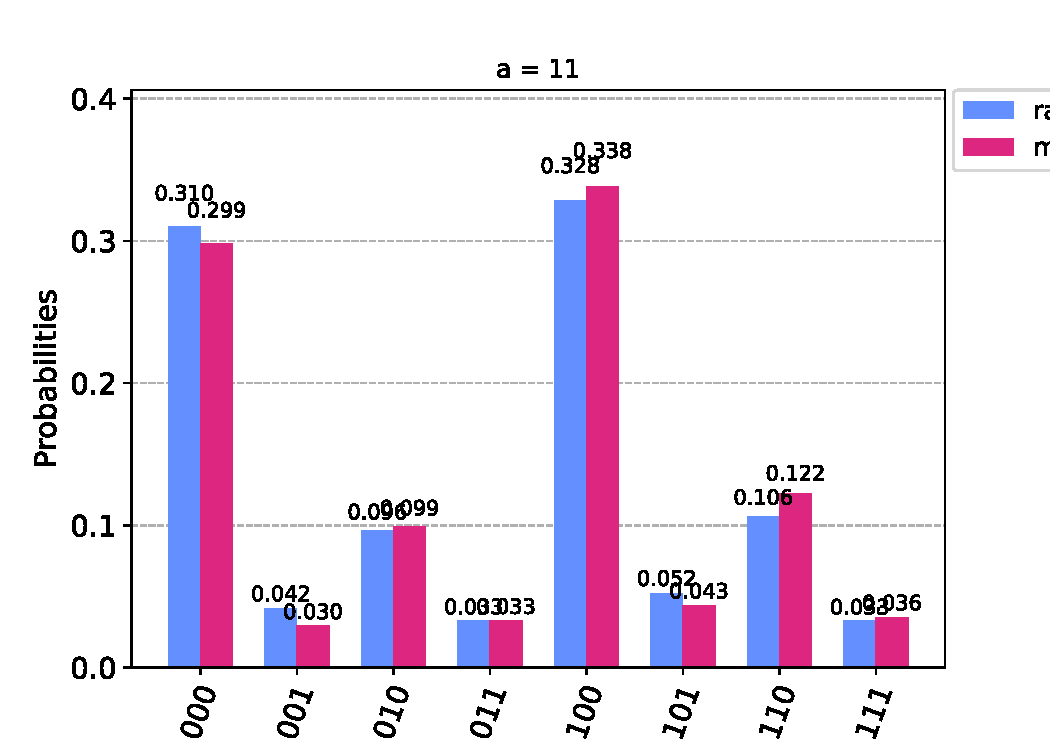
\includegraphics[width=0.8\linewidth]{./figs/error_mitigation_11_cambridge.pdf}
	\end{figure}
\end{frame}

\begin{frame}{Results}
	\begin{figure}[h]
		\centering
		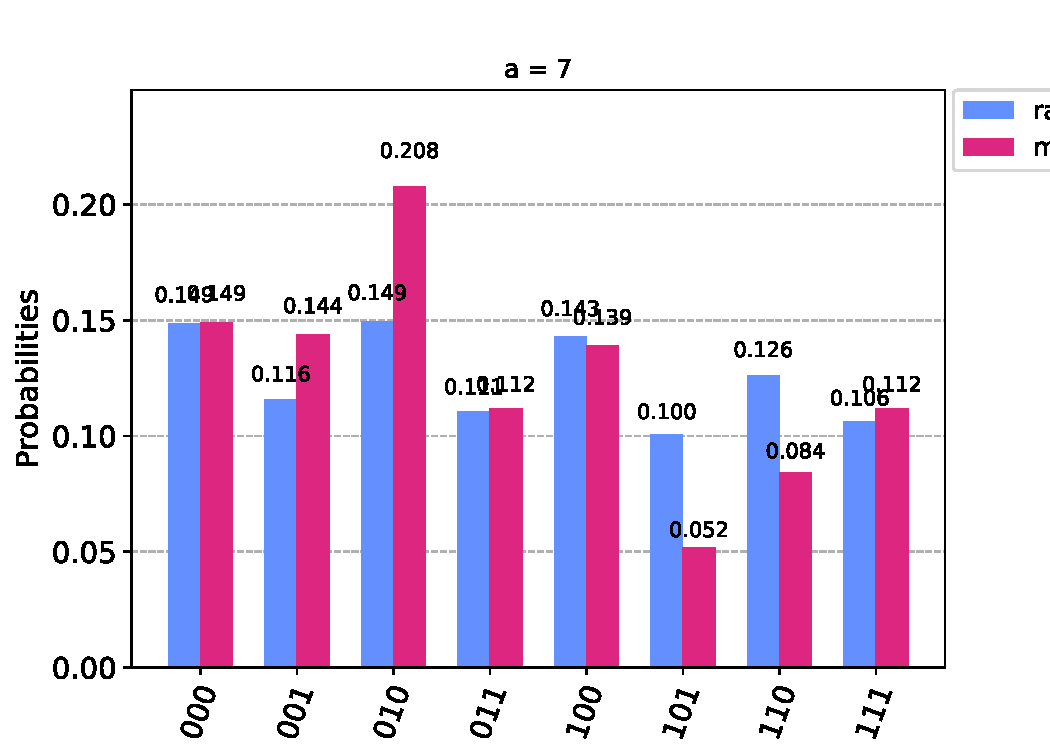
\includegraphics[width=0.8\linewidth]{./figs/error_mitigation_7_rochester.pdf}
	\end{figure}
\end{frame}

\begin{frame}{Results}
	\begin{figure}[h]
		\centering
		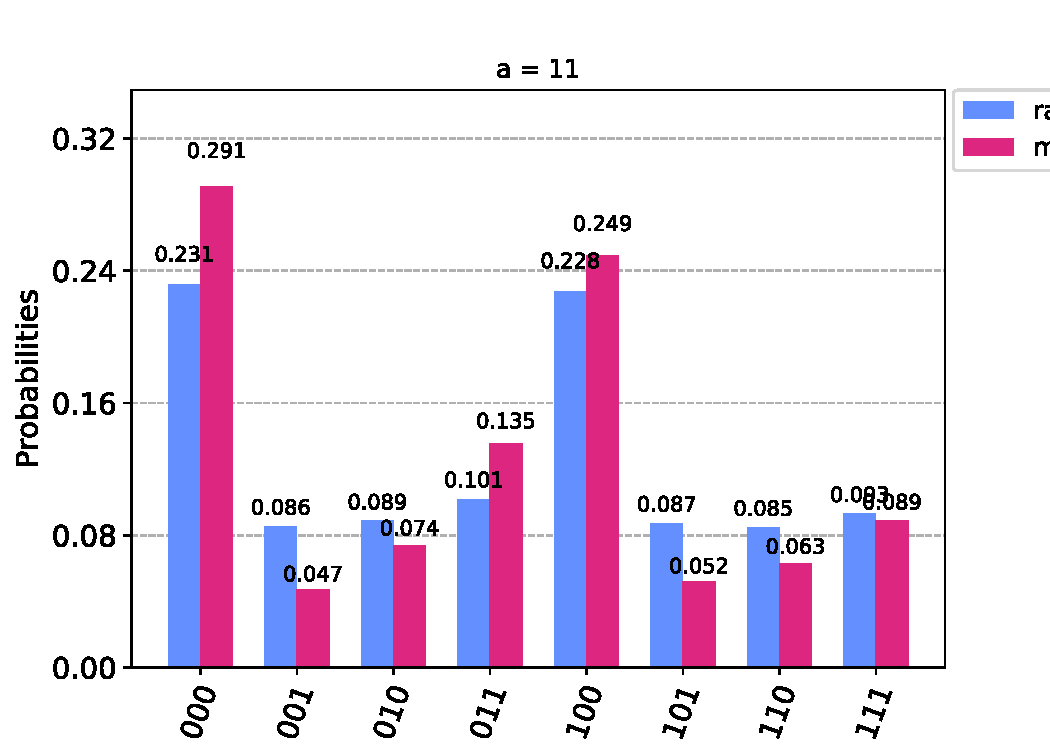
\includegraphics[width=0.8\linewidth]{./figs/error_mitigation_11_rochester.pdf}
	\end{figure}
\end{frame}

\begin{frame}{Results}
	\begin{figure}[h]
		\centering
		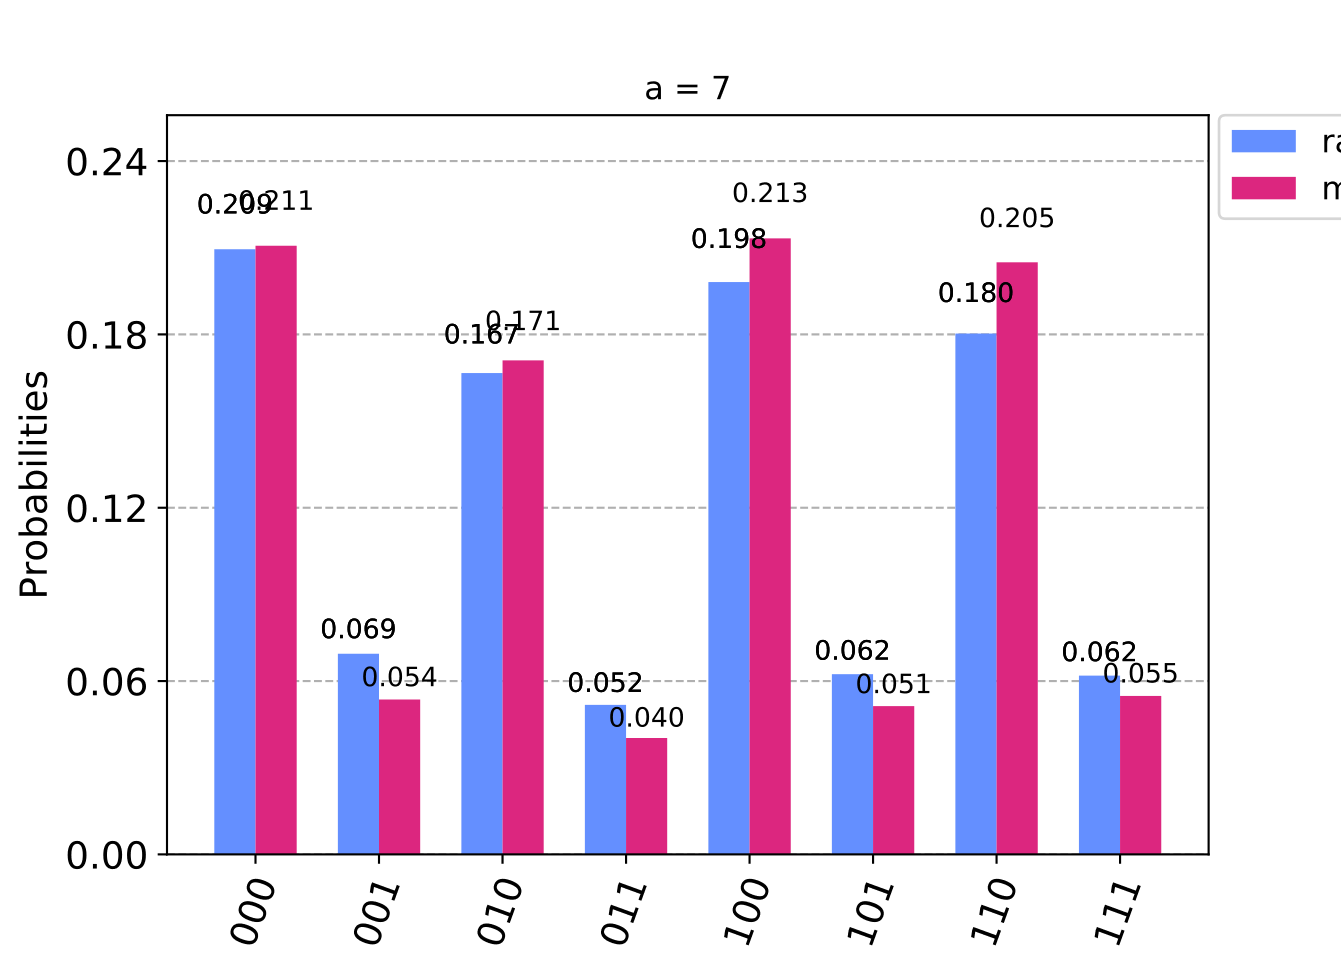
\includegraphics[width=0.8\linewidth]{./figs/error_mitigation_7_cambridge_2.png}
	\end{figure}
\end{frame}

\begin{frame}{Results}
	\begin{figure}[h]
		\centering
		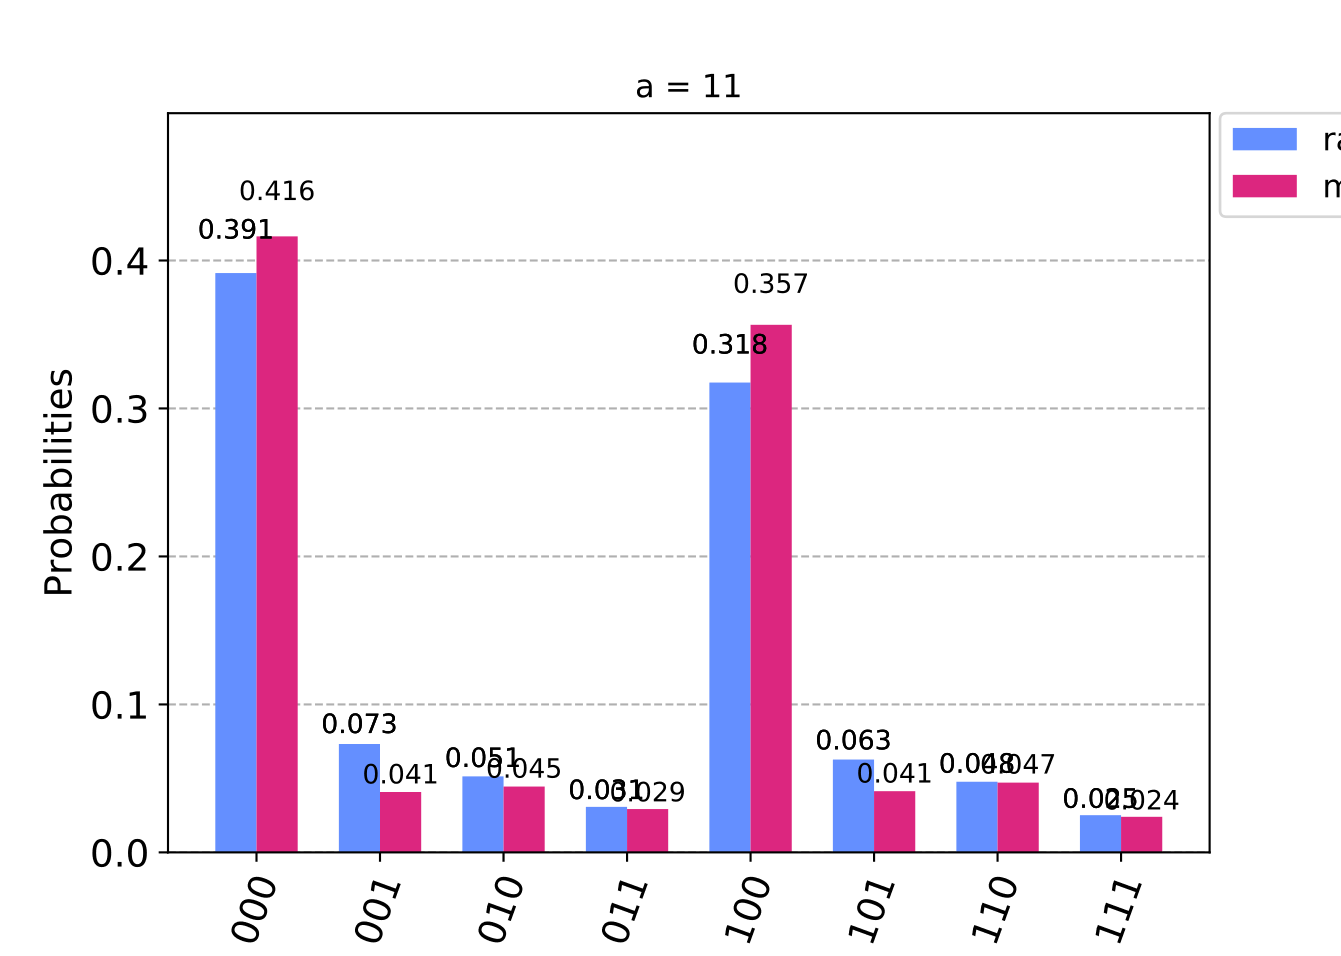
\includegraphics[width=0.8\linewidth]{./figs/error_mitigation_11_cambridge_2.png}
	\end{figure}
\end{frame}

\begin{frame}{Discussion}
	The result was not well. What was causing the error? Depth?
	What determines the depth?
	\begin{itemize}
		\item Hardware
		\item Transpiler/compiler
	\end{itemize}
\end{frame}

\begin{frame}{Hardware}
	\begin{figure}[h]
		\centering
		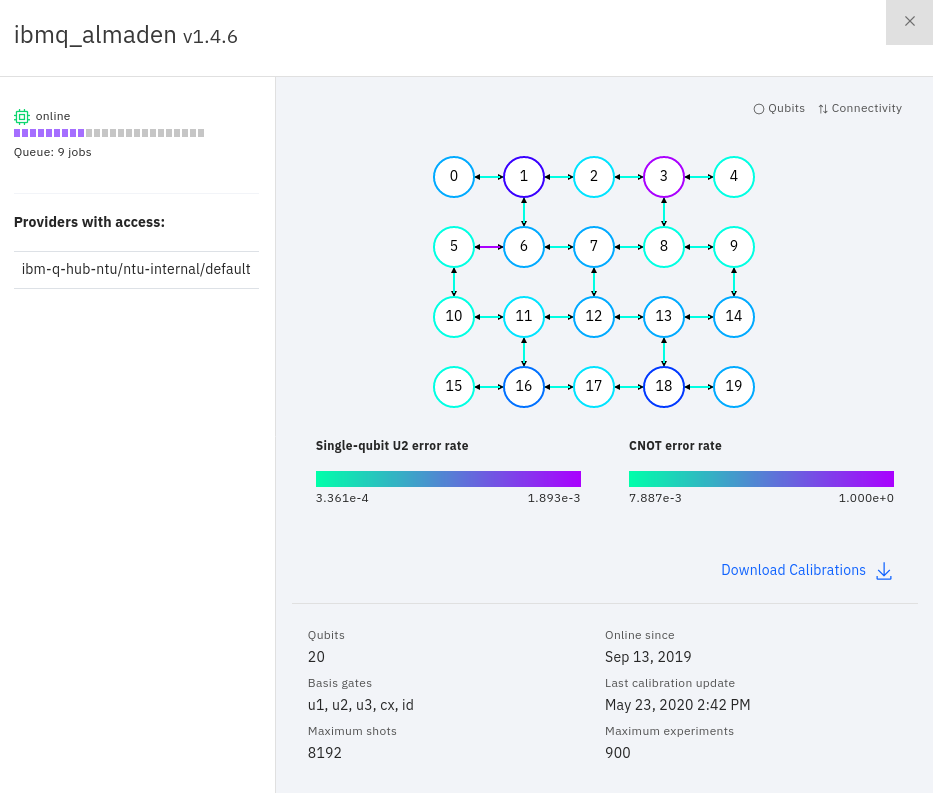
\includegraphics[width=0.8\linewidth]{./figs/hardwareexample.png}
	\end{figure}
\end{frame}

\begin{frame}{Transpiling/compiling}
	Use \texttt{qk.compiler.transpile(qc, backend=be, initial\_layout=layout,
	optimization\_level=1)} to assign manually.
	\begin{figure}[h]
		\centering
		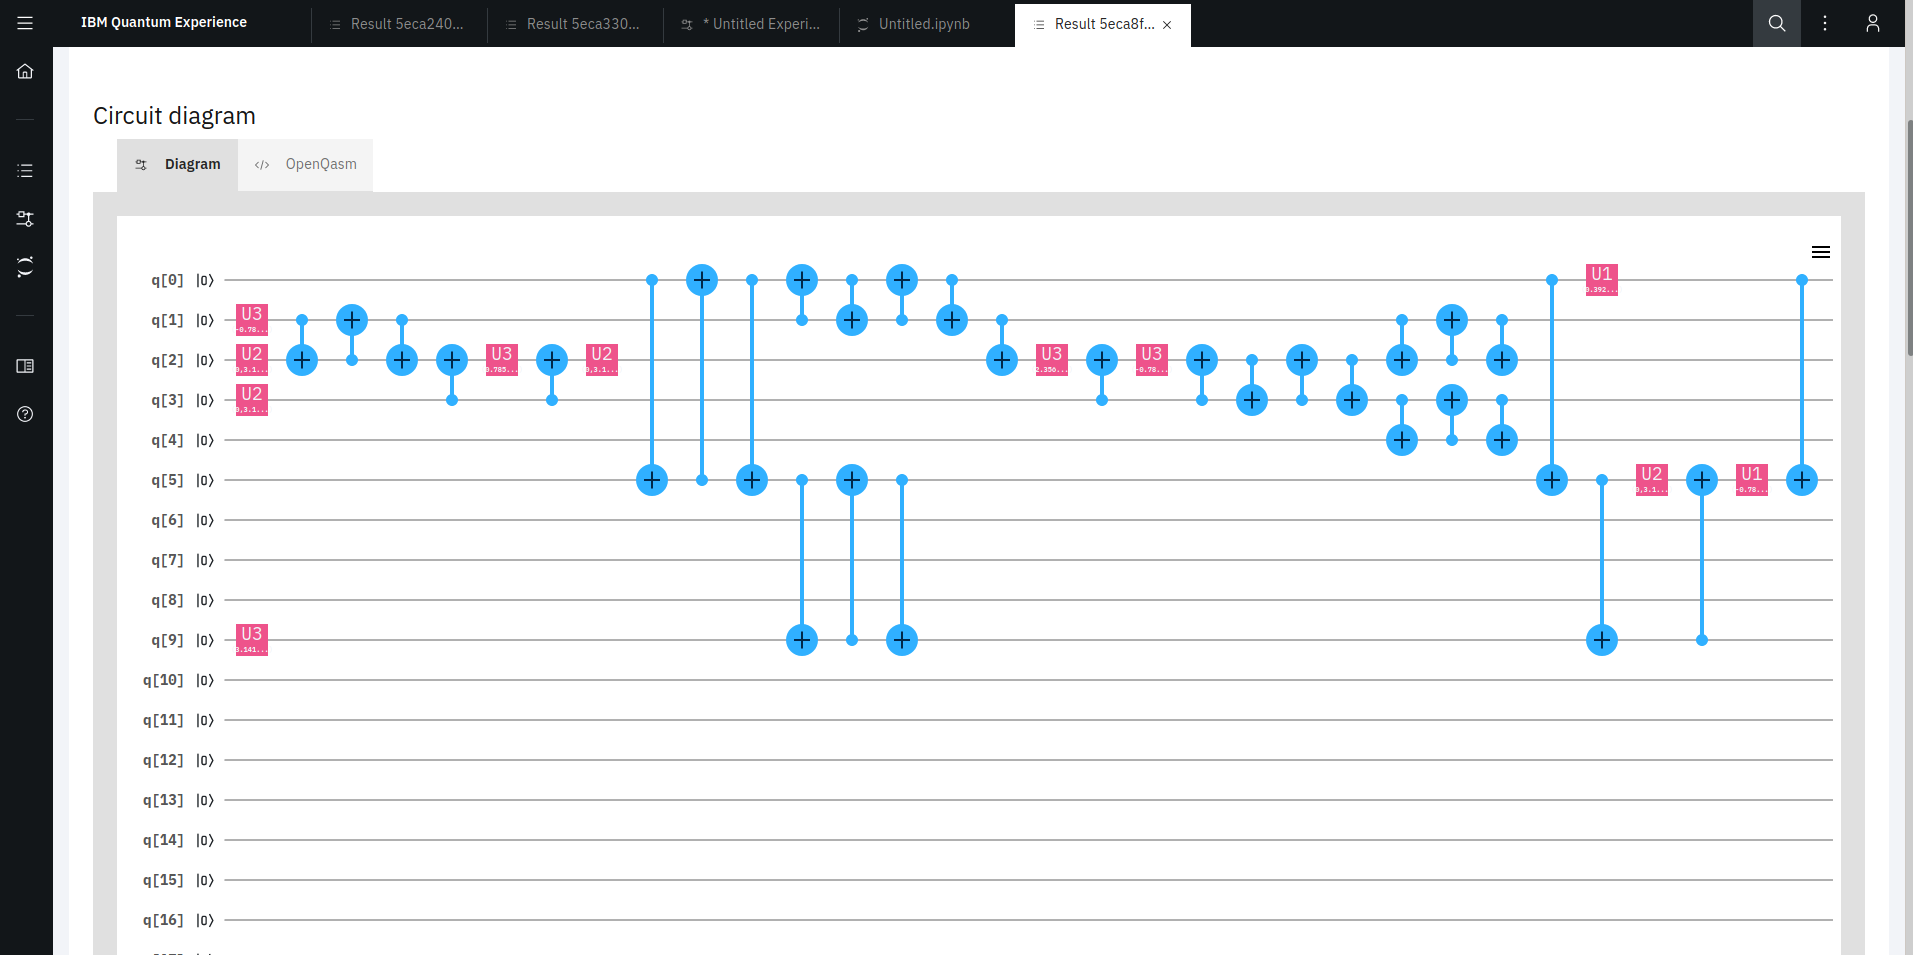
\includegraphics[width=\linewidth]{./figs/circuitdiagramexample.png}
	\end{figure}
\end{frame}

\subsection{Depth vs. Error}%
\label{sub:depth_vs_error}

\begin{frame}{Depth vs. error}
	\begin{itemize}
		\item Obviously $\text{depth}\uparrow \Rightarrow \text{error} \uparrow$
			\begin{itemize}
				\item But quantitatively?
			\end{itemize}
		\item Create random circuits to test errors!.
		\item What to expect? Exponential decay of accuracy.
	\end{itemize}
\end{frame}

\begin{frame}{Depth vs. error: random circuits}
	\begin{figure}[h]
		\centering
		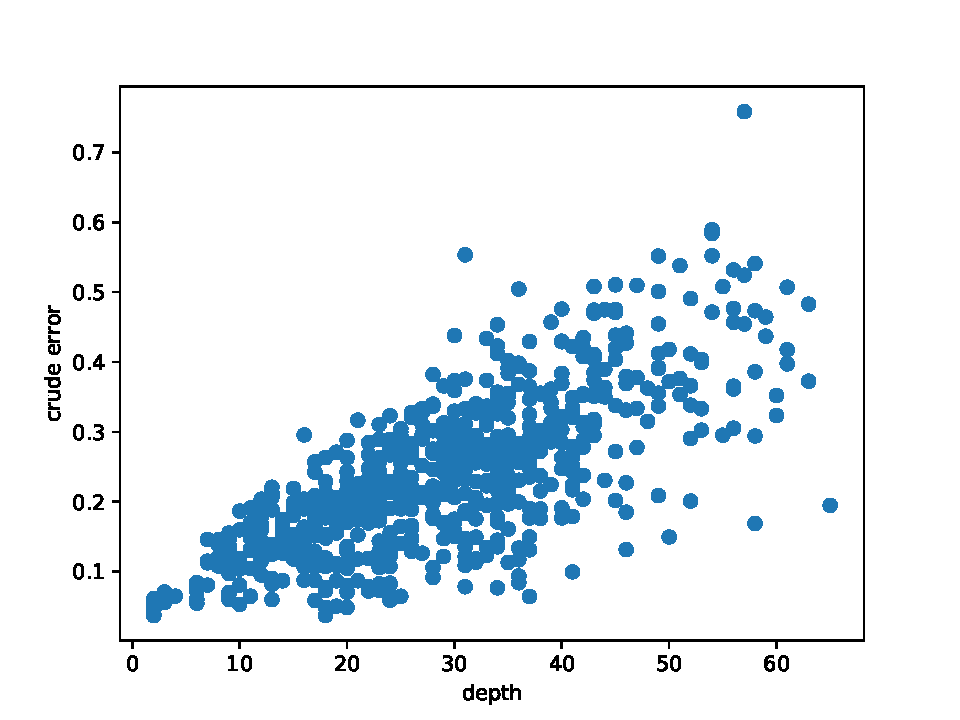
\includegraphics[width=0.8\linewidth]{./figs/depth.pdf}
	\end{figure}
\end{frame}

\begin{frame}{Discussion}
	\begin{itemize}
		\item Bad definition of error!
		\item Use a circuit with definite results.
	\end{itemize}
\end{frame}

\begin{frame}{Depth vs. error: adder}
	\begin{figure}[h]
		\centering
		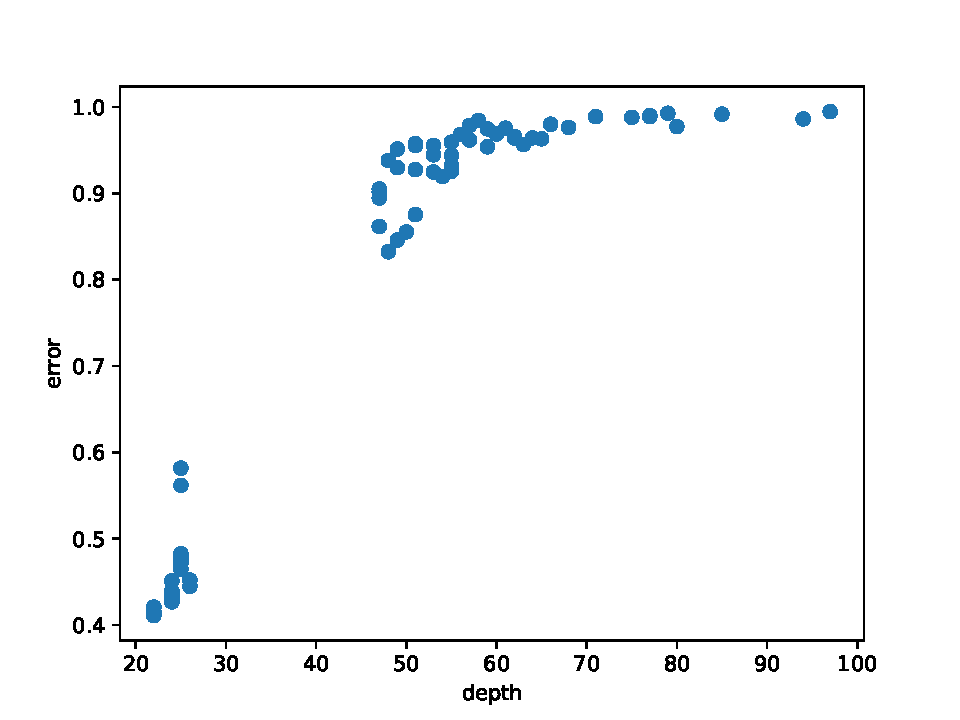
\includegraphics[width=0.8\linewidth]{./figs/adder_error.pdf}
	\end{figure}
\end{frame}

\begin{frame}{Depth vs. error: adder}
	\begin{figure}[h]
		\centering
		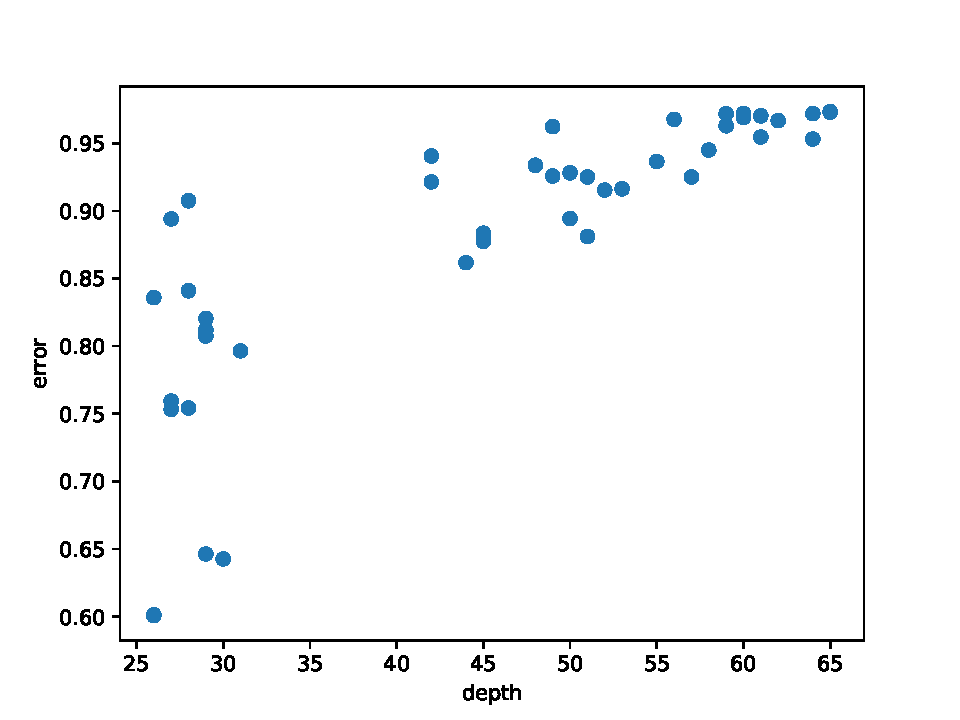
\includegraphics[width=0.8\linewidth]{./figs/adder_error2.pdf}
	\end{figure}
\end{frame}

\end{document}
